\onecolumn
\fontsize{12pt}{12pt}\selectfont
\fancyhf{}
\setcounter{page}{4}
Links for the task:
\begin{enumerate}
    \item \href{https://kvant.ras.ru/1971/10/p59.htm}{Main page}.
    \item \href{https://kvant.ras.ru/1971/10/p51.htm}{Table is here}.
    \item \href{https://kvant.ras.ru/1970/07/p37.htm}{Additional task}.
    \item \href{https://github.com/GreatAccName/itmo-1infa-lab6.git}{My GitHub Repository}.
\end{enumerate}
Additional tasks: $\Sigma_{b={1}}^\infty \frac{b^2\sqrt{3}}{4}$;
\[
    \sum_{b=0}^\infty \frac{b^2\sqrt{3}}{4}.
\]

\usetikzlibrary{arrows,snakes,backgrounds,positioning}
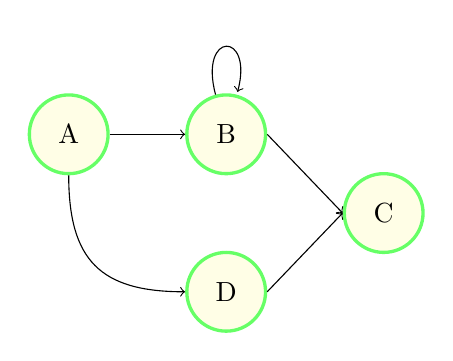
\begin{tikzpicture}[
roundnode/.style={circle, draw=green!60, fill=yellow!10, very thick, minimum size=10mm}
]
    \node[roundnode] (nodeA) at ( 0,2) [shape=circle,draw] {A};
    \node[roundnode] (nodeB) at ( 2,2) [shape=circle,draw] {B};
    \node[roundnode] (nodeC) at ( 4,1) [shape=circle,draw] {C};
    \node[roundnode] (nodeD) at ( 2,0) [shape=circle,draw] {D};

    \draw[->] (nodeA.east) -- (nodeB.west);
    \draw[->] (nodeB.east) -- (nodeC.west);
    \draw[->] (nodeD.east) -- (nodeC.west);
    \draw [->] (nodeA) .. controls +(down:16mm) and +(left:16mm) .. (nodeD);
    \path (nodeB) edge [loop above] node {} (nodeB);
\end{tikzpicture}